\section{Technical Development}
\subsection{User Interface Design}
The User interface for this project is designed after looking at the user interfaces used by other music applications. In particular, the developer was inspired by Spotify, shown in figure \ref{fig:spotify}.

\begin{figure}[h]
    \centering
    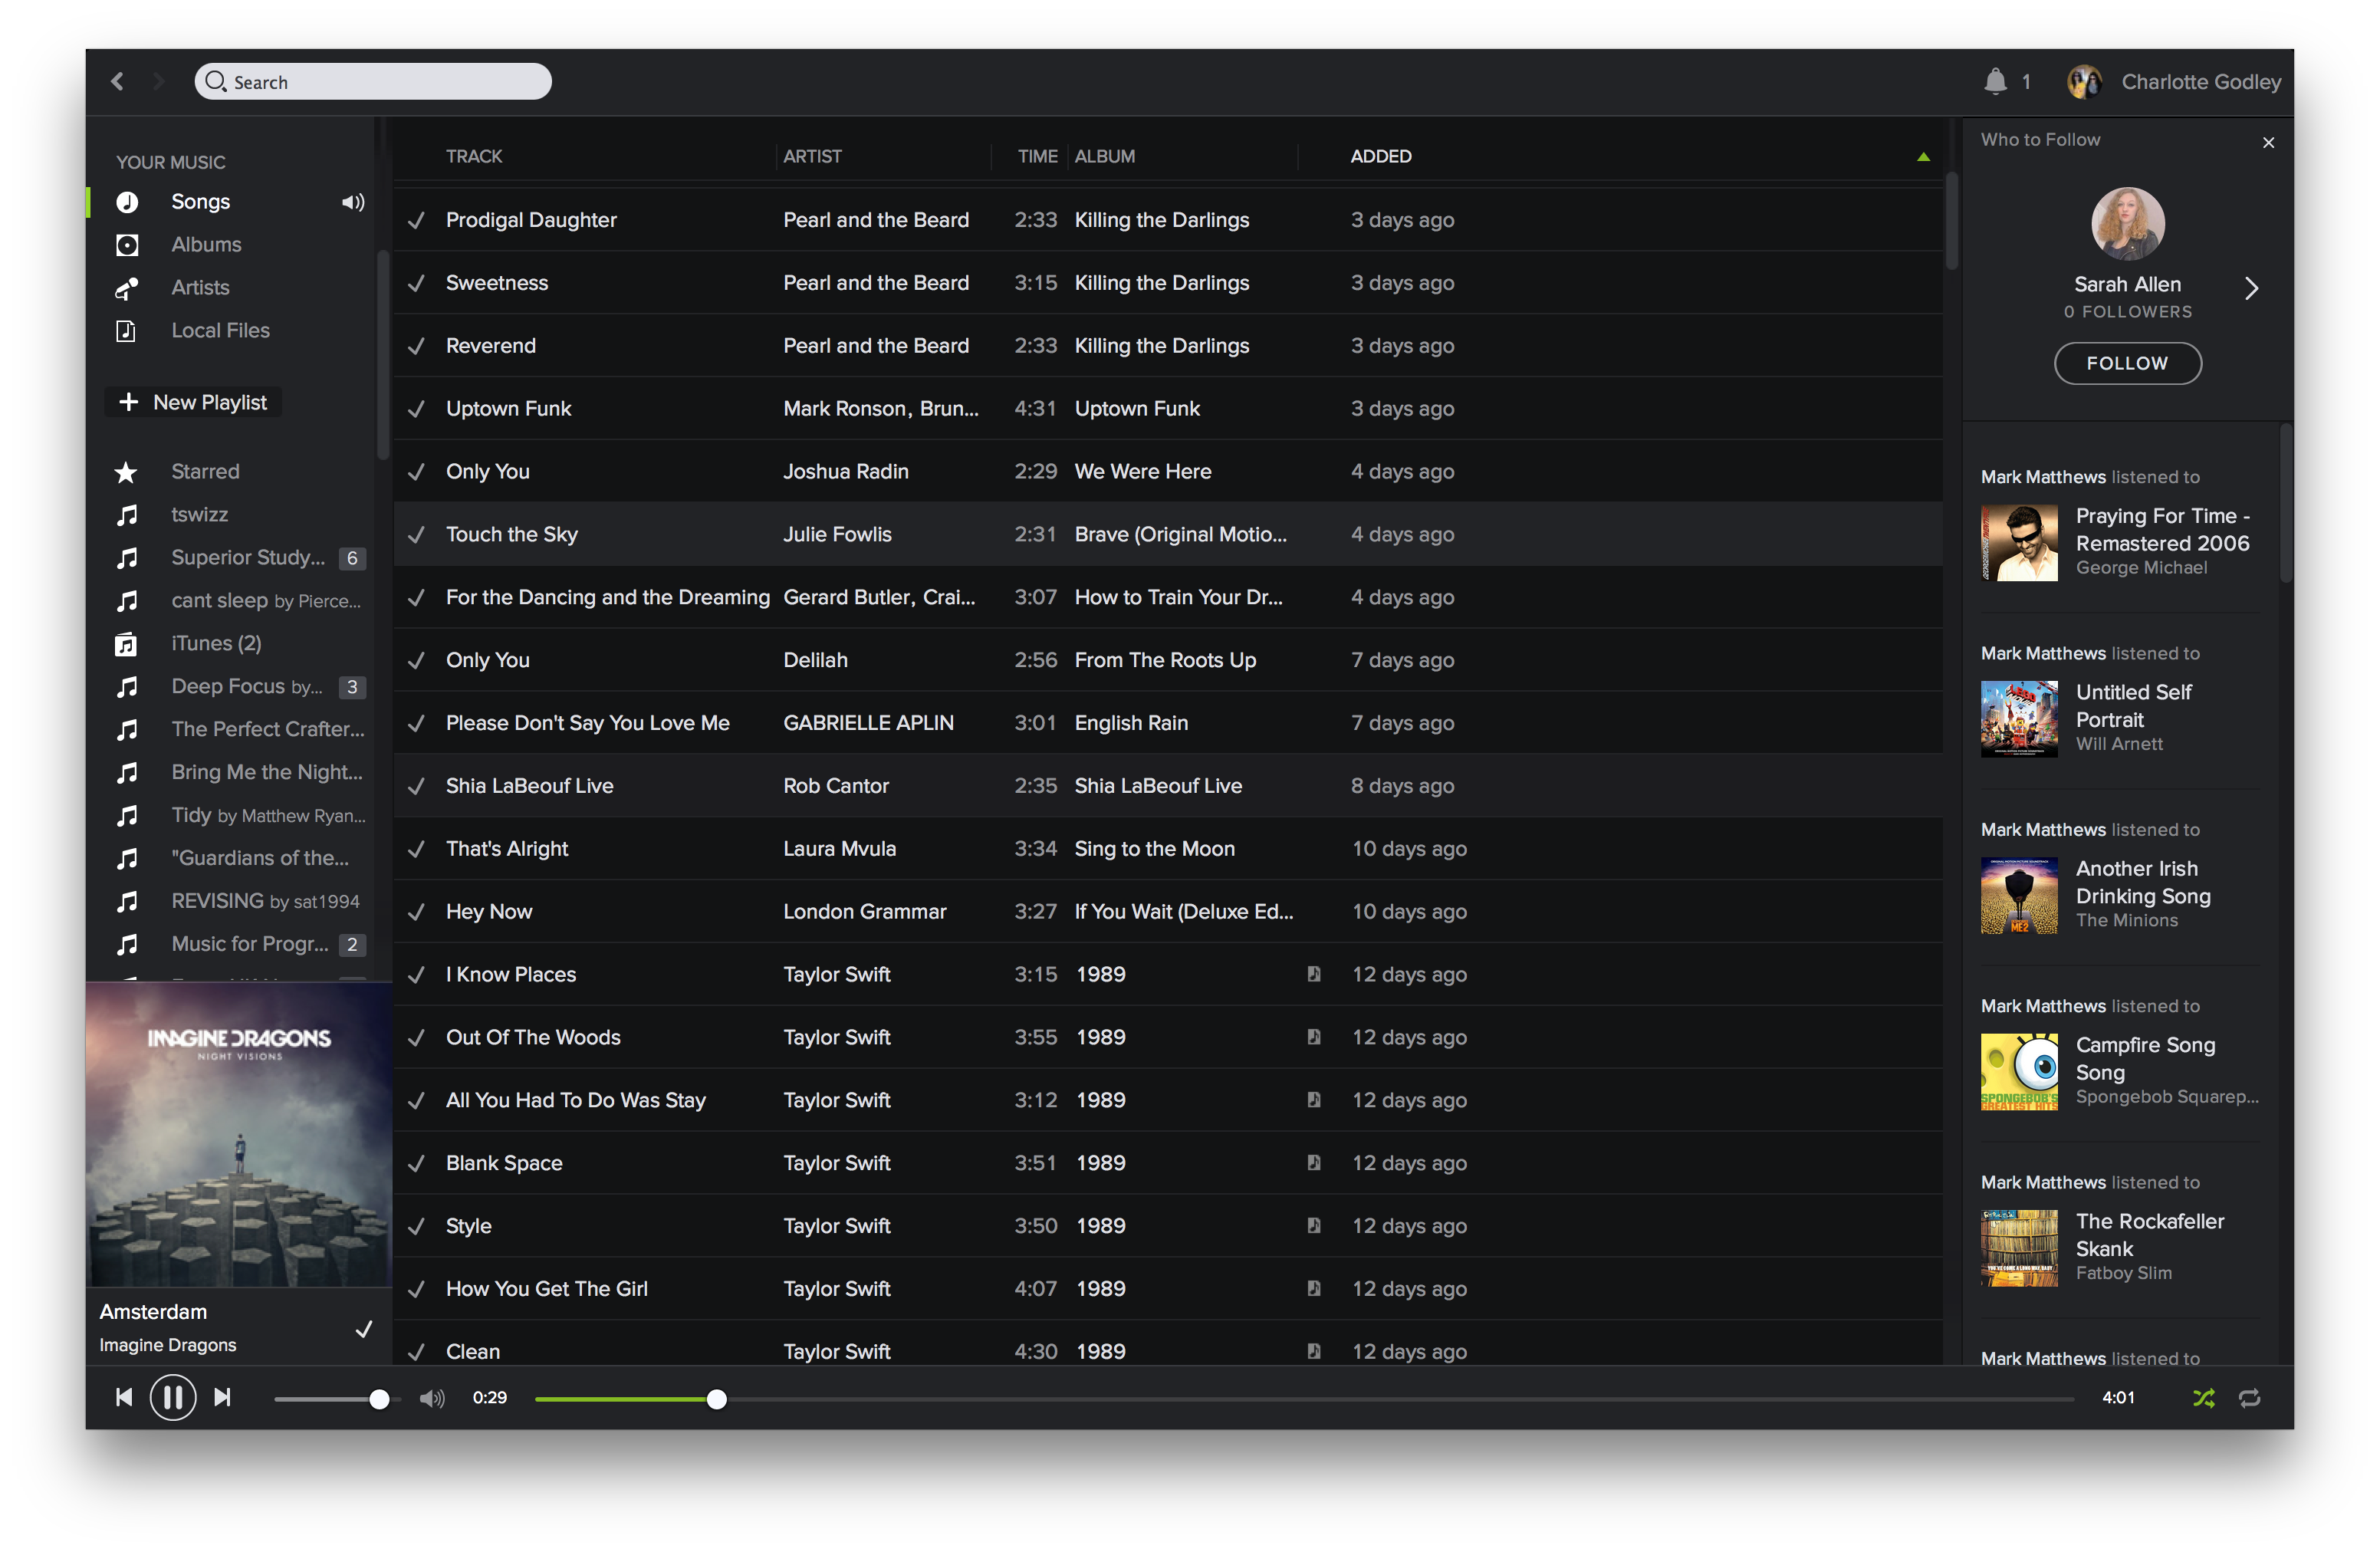
\includegraphics[width=\textwidth]{screen.png}
    \caption{Spotify user interface}
    \label{fig:spotify}
\end{figure}
\subsubsection{Main Display}
\begin{figure}[H]
    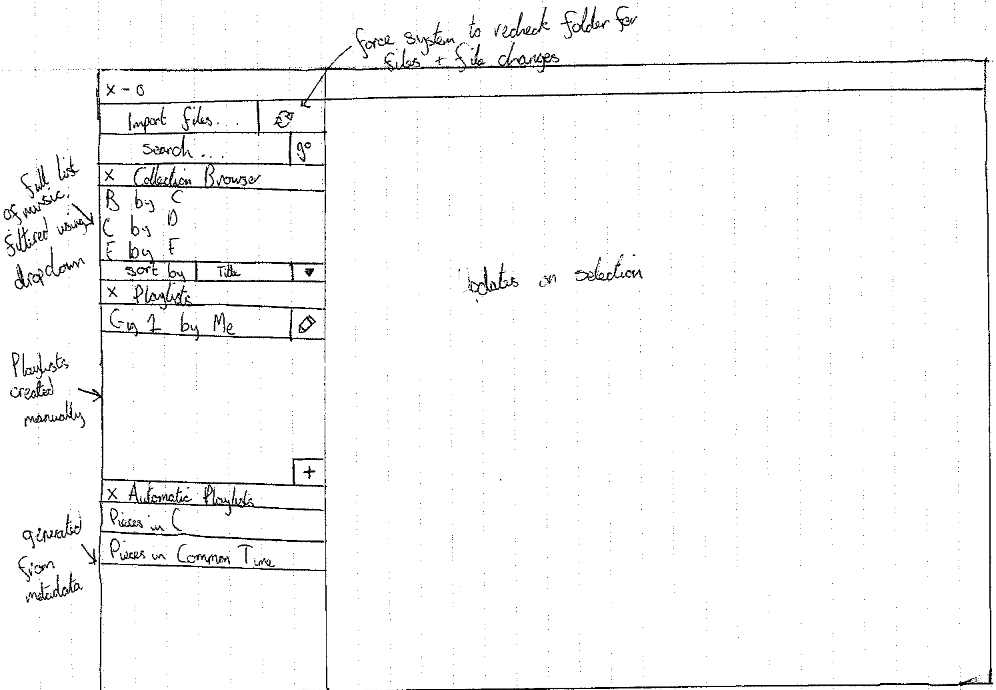
\includegraphics[width=400pt]{designs/main}
    \caption{Main User interface of the project}
    \label{fig:main}
\end{figure}
Figure \ref{fig:main} shows the main view of the application. Various panes to the left can be closed using the X button and show different ways the music can be displayed, either as individual units or as playlists. The larger pane next to it shows the area in which sheet music or a list of pieces in a playlist will be displayed, depending on the selection from the left pane. Updates to this and pop up boxes displaying dependent on buttons in the window are displayed and explained in the appendices.

\subsection{Test Design and System Testing}
This project was developed using Test Driven Development. This is an Agile software development methodology which utilises the rules that a line of code should not be written unless there is a failing automated test \parencite{TDD}. This methodology has been chosen as the nature of the notation of music means that meticulous detail must be payed to how and with what symbol every element is notated, and Test Driven Development will significantly improve the quality of the software by closely integrating testing with the development process.

As such, no test design or plan was produced, but rather tests were developed as features were introduced, and were designed to be self contained units testing the smallest possible details, such as an accent being added to a measure correctly, or a note's pitch being created with a particular note name or octave number.

Test cases were created using the aforementioned software MuseScore. These were produced by creating a file for every area of notation (e.g. clefs, time signatures, note durations, pitch) and applying each and every symbol possible within that area to the music. It was decided to create test cases in this way to thoroughly ensure that no piece of notation was missed. An example testcase, and a list of all testcases in use and their value in real world testing, are included in the appendices.

Further to the testcases developed specifically for this application, the system was tested against a larger set of tests called "The Unofficial MusicXML testsuite", which was released by the Lilypond Project to provide a comprehensive test suite for all elements of MusicXML\parencite{LilypondTestcase}. 

\subsubsection{User Testing}
In order to understand how well this user interface works with a variety of users, a survey was designed which will be given to a selection of musicians, who will feedback on how easy the UI is to use and any updates which should be made to improve it. This feedback session will be performed after the initial sketches are made into a virtual user interface with no back end connected to the buttons. An example survey is provided in the appendices.

\subsection{System Design}
\subsubsection{Overall Architecture}
The flow chart in figure \ref{fig:flowchart} was designed prior to developing any code, in order to visualise how the objectives would interlink with each other.
\begin{figure}[H]
    \centering
    \includegraphics[width=400pt]{diagrams/overall_system.pdf}
    \caption{A flow diagram describing the project}
    \label{fig:flowchart}
\end{figure}

\subsubsection{Metadata Scanning system}
The flow diagram in \ref{fig:flowchart} refers to applying a metadata scanning system to the folder. This is described in more detail in the flow diagram in figure \ref{fig:meta}. 
\begin{figure}[H]
    \centering
    \includegraphics[width=250pt]{metadata_algorithm-crop}
    \caption{A flow diagram describing the meta scanning system}
    \label{fig:meta}
\end{figure}
\subsubsection{Metadata Class Structure}
The metadata scanning objective implements the popular Model View Controller design pattern, which separates the user interface (view) from the program logic (controller) and any databases or information storage (model). %todo ref
In this instance as shown in the class diagram in figure \ref{fig:metadiagram}, the music manager class acts as the controller, which takes input from the application interface and request data from the data layer, which interacts with an SQLite file.

The decision was taken to use this pattern in order to avoid coupling to any particular database and to ensure that the objective was properly organised according to functionality. This decision was also influenced by considerations about the future of the project.

\begin{figure}[H]
    \centering
    \includegraphics[width=\textwidth]{diagrams/api_and_meta_data_diagram}
    \caption{Metadata and API Class Diagram}
    \label{fig:metadiagram}
\end{figure}

\subsubsection{Modular Design}
The MVC design pattern was complemented by the implementation of the  modular design pattern, in which functions and collections of functions are separated into independent blocks or modules. %todo ref
This is shown in the class diagram in figure \ref{fig:metadiagram} as the music manager also interacts with other classes such as the folder browser, which handles all functionality involving scanning the given folder for new, old, or zipped files, and the unzipper, which handles the functionality for manipulating zip files.

It is also present in the rendering system explained in detail in section 4.3.5, as each section of the object hierarchy collects its own Lilypond formatting, and then calls upon its child classes to collect theirs, finally collaborating into one complete Lilypond file. In the context of sheet music this is particularly important, as symbolic notation has many options for symbols which may or may not be present, so in program logic they must all act independently of other symbols occurring in the file.

This design was influenced by the decision to use test driven development, as this development methodology aims to test small units of program functionality in an isolated environment. %todo ref
 As such, this was easier to achieve if each independent class had one role in the system, with management classes handling the collaboration of these roles without needing to test multiple elements of functionality at once. 

This makes the code and overall architecture reusable in different situations. For example, the API manager class sends data collected online back to the Music Manager, which can then communicate with the metadata scanner to extract further information, which avoids code duplication.

\subsubsection{Rendering Architecture}
The class diagram in figure \ref{fig:classdiagram} shows an abstract structure of the sheet music rendering implementation used in this project. This implements a tree, each node of which holds an item containing the notation specific to that node. Each item object and node object implements the ToLily method which outputs that node, node item and children's collateral lilypond-formatted string. A tree was chosen as the object structure in order to give an indication of time, and in order that specific elements could be positioned according to sequential instructions from the MusicXML parser. 
\begin{figure}[H]
    \centering
    \includegraphics[width=\textwidth]{diagrams/class_diagram_drawing}
    \caption{Renderer Class Diagram}
    \label{fig:classdiagram}
\end{figure}
\subsubsection{Duck Typing}
The rendering system visualised by figure \ref{fig:classdiagram} implements a feature of dynamic typing known colloquially as Duck Typing. %todo ref

In respect to the rendering system, this means that each class assumes its child classes, if any are present, have the ToLily method, call the method and collaborate the results. Defining classes by their behaviour, not their attributes is important to the project as this avoids assumptions about what the music will or will not contain. 

It also means that future feature implementations or symbols which are added to the renderer need only implement a ToLily method and be linked into the input parser scripts in order to be implemented in the rendered output.

\subsubsection{Designing for extensibility}
This project is designed with a particular aim of extensibility. This affects each area of the system in a different way, but in general, it means that the elements in the system are able to be modified, improved or expanded without requiring changes to the organisation of the system. 

An example of this is the API manager, which holds a dictionary of sources, with each index pointing to a class. The API manager will cycle through these sources when its methods are called, meaning that to implement a new API, the developer would simply put a new entry into this dictionary.

Each source implements the API class. To avoid causing problems with classes missing particular methods, the API class will throw a not implemented exception if the sub class does not override the method, in order to indicate to the developer working with a new API that this method is necessary.


\subsection{System Implementation}
\subsubsection{Development Methodology}
The project was implemented using a developer informed process, whereby the developer would review the project's status for bugs, issues and features which had yet to be implemented, note this using an issue tracker, select an issue based on the priorities of the project, develop tests for this issue and finally, develop the production code. 


Issue tracking and reporting was used so that the developer could think and reflect on areas of the system which needed improvement, modification or implementation. The methodology worked well in the context of a year long project in which development was not continuous because it ensured that when development was paused, the developer could see instantly what needed to be doing or what was being worked on before the pause to work on something else. 

This adds the benefit that in the future, when this project may be worked upon by more than one developer, new developers can see things which have yet to be implemented and choose which features are most relevant or doable by their own standards, as well as discuss or contest previous issues in the system.


\subsubsection{Challenges in the rendering system}
The renderer in this project was designed around two open formats - MusicXML and Lilypond. Whilst every effort was made to avoid coupling with either format, designing the system to work seamlessly with both formats was difficult, and many problems were encountered structuring the object format.

Initially, the project used a simpler object structure in which measures contained a list of items contained within that measure. This was due to MusicXML items having no unique identifiers which could be used to indicate at which point they occurred within that measure, so objects had to be loaded and stored sequentially.

It was then discovered that Lilypond dictates that dynamics and some other elements, which are classed as directions in MusicXML, had to occur directly after the note to which they should be assigned %todo ref
. This meant that the structure had to be redesigned to classify notes as first class objects, for which other elements would be indexed according to which note they occurred after, and that directions and "expressions" as Lilypond refers to them as needed to be split into two lists, in order to ensure that expressions could be put before directions, but not before the note they should be assigned to.

Later it was discovered that MusicXML allows for navigation through a measure using two specific tags called "forward" and "backup", which in the original system would require a lot of list manipulation to position elements correctly. 

Various other feature inclusions led to the developer redesigning the system around these factors, finally reaching the tree structure described in the design section. This enabled the developer to move objects around according to the tags which next occurred.

Fundamentally, the difference in the design aims for MusicXML and Lilypond is that MusicXML dictates a sheet music file by how it appears, as in the above example, sequentially positioning the elements is how a viewer would see the overall piece. Lilypond, on the other hand, dictates a sheet music file by how it is played - after all, a dynamic without a note would not achieve the desired result as these dictate the volume of a particular element, or elements, of music. 

There are many other examples of this throughout both formats, and all of these affected the development time of the first objective adversely. Redesigns and refactors were made at late stages of development due to it being virtually impossible to know all of the nuances of such complex formats without working with them intensively. It may have been a suggestion to extend the research period before development to accommodate this, but a research period long enough to understand the design aims of the formats in enough detail to design the structure in the initial stages would have taken away valuable development time.

\subsubsection{Use of external technologies and libraries}
For this project, external libraries were used for the graphical user interface and for the database layer. Both were necessary to avoid development duplication and will be discussed in the sections below.

\textbf{User interface libraries} \\
There are several libraries available for creating a graphical user interface in Python, with the most popular ones summarised in table \ref{table:gui}.

\begin{table}[H]
\centering
\begin{tabu} to 1.05\textwidth {| l | l | l | l |} \hline
  {Library} & {Benefits} & {Drawbacks} & {Cross platform} \\ \hline
  Qt & Has its own designer (QtDesigner) and some other third party designers & Long installation process \\
   &  popular amongst many languages & no built in PDF viewer\\
   &  can use CSS to style widgets \\
  & & & \checkmark \\ \hline
  Wx 
  & Built in PDF display & Designers not as powerful as Qt + all are third party & \checkmark \\ 
  & several designers made for it \\ \hline
  TKinter & Built into Python itself & No designers\\ 
  & & No built in PDF/PNG viewers\\
  & & Binds to an old language which is rarely updated & \checkmark \\ \hline
  AppKit & Works well on OSX & Not cross platform &  $\times$ \\ \hline
  
\end{tabu}
\caption{Table of GUI libraries in python}
\label{table:gui}
\end{table}

Python as a language is cross platform, which is one of the reasons for its popularity, and as such there is only one library in popular usage (AppKit) which is locked to one platform, as shown by the table.

In the initial phases of GUI prototyping, the developer worked with each of the other options in turn and dismissed each one, apart from Qt which the GUI is written in, for various reasons.


The first trial was TKinter, being as it is built into the Python library and did not require any installation. TKinter is a library which provides a python binding to TCL's user interface libraries. %todo ref
 These have not been updated or upgraded for today's image formats, and do not support PDF or PNGs. Any use of either of these formats required installation of other libraries, such as the Python Image Library (PIL). %todo ref
 Furthermore, as discussed by \cite{GuiProgramming}, there are very few open, non-commercial options for graphical GUI designers for TKinter, meaning that any interfaces had to be hard coded using python code, rather than creating designed files to be imported.
 
 The second trial was 
 
 The third and final trial was Qt. This library took longer to install, being as PyQt, like TKinter, is only a binding to a lower level C++ library. This means that PyQt cannot be installed in the same way as Wx, using the Python Package Library pip, and for windows meant installing and compiling all sections of PyQt, Qt and SIP which links the two together from source, as no pre compiled installer was available.
 
 In addition to this development time, Qt does not provide a widget for PDF documents, which meant the developer installed a second third party library called Poppler, which is also a C++ library with Python bindings. This library was found to be far easier to use than the Python Image Library used by TKinter.
 
 Whilst this extended the time taken to produce a fully cross platform application installer, Qt provides a fully extensible QtDesigner application, which enables developers to produce their designs, including applying CSS to widgets, in a graphical user interface which outputs UI xml files. 
 
 The xml files are then loaded into Python, meaning that any changes to the files through the designer automatically affect the python binding the next time the developer runs the application.

Furthermore, as Qt is a common library to other languages and is reasonably popular, far more support was found for installing, using and extending Qt than the other libraries the developer tried to use, so the developer decided to use Qt.

\textbf{Databases and Database Libraries}
Table \ref{table:databases} shows the options for databases the developer could have implemented in this project.

\begin{table}[H]
\centering
\begin{tabular}{| l | l | l |} \hline
  {Library} & {Benefits} & {Cross platform} \\ \hline
  Qt & Has its own designer (QtDesigner) and some other third party designers & Yes \\ \hline
  Wx & Built in PDF display, several designers made for it & Yes \\ \hline
  TKinter & Built into Python itself & Yes \\ \hline
  AppKit & Works well on OSX & No \\ \hline
  
\end{tabular}
\caption{Table of GUI libraries in python}
\label{table:gui}
\end{table}

